The first model is used as an initial approach to the problematic.
\begin{center}
    \begin{verbatim}
    Model: "sequential"
    _________________________________________________________________
    Layer (type)                 Output Shape              Param #   
    =================================================================
    conv2d (Conv2D)              (16, 32, 32, 32)          320       
    _________________________________________________________________
    conv2d_1 (Conv2D)            (16, 32, 32, 32)          9248      
    _________________________________________________________________
    max_pooling2d (MaxPooling2D) (16, 16, 16, 32)          0         
    _________________________________________________________________
    conv2d_2 (Conv2D)            (16, 16, 16, 64)          18496     
    _________________________________________________________________
    conv2d_3 (Conv2D)            (16, 16, 16, 64)          36928     
    _________________________________________________________________
    max_pooling2d_1 (MaxPooling2 (16, 8, 8, 64)            0         
    _________________________________________________________________
    conv2d_4 (Conv2D)            (16, 8, 8, 128)           73856     
    _________________________________________________________________
    conv2d_5 (Conv2D)            (16, 8, 8, 128)           147584    
    _________________________________________________________________
    max_pooling2d_2 (MaxPooling2 (16, 4, 4, 128)           0         
    _________________________________________________________________
    flatten (Flatten)            (16, 2048)                0         
    _________________________________________________________________
    dense (Dense)                (16, 128)                 262272    
    _________________________________________________________________
    dense_1 (Dense)              (16, 10)                  1290      
    =================================================================
    Total params: 549,994
    Trainable params: 549,994
    Non-trainable params: 0
    _________________________________________________________________
    \end{verbatim}
\end{center}
The network is defined to be optimized using the Adam algorithm\footnote{\href{https://keras.io/api/optimizers/adam/}{https://keras.io/api/optimizers/adam/}},
choosing the following hyperparameters:
\begin{itemize}
    \item learning\_rate = 0.001
    \item beta\_1 = 0.9
    \item beta\_2 = 0.999
    \item epsilon = 1e-07
    \item amsgrad = False
\end{itemize}
The chosen loss function to optimize is Cross Entropy\footnote{\href{https://www.tensorflow.org/api\_docs/python/tf/keras/losses/CategoricalCrossentropy}{https://www.tensorflow.org/api\_docs/python/tf/keras/losses/CategoricalCrossentropy}}
(especially defined for One-Hot encoded outputs).\\
Training this model on the prepared dataset gives us an accuracy of approximately 60\%, which is good but improvable:
\begin{center}
    \captionsetup{type=figure}
    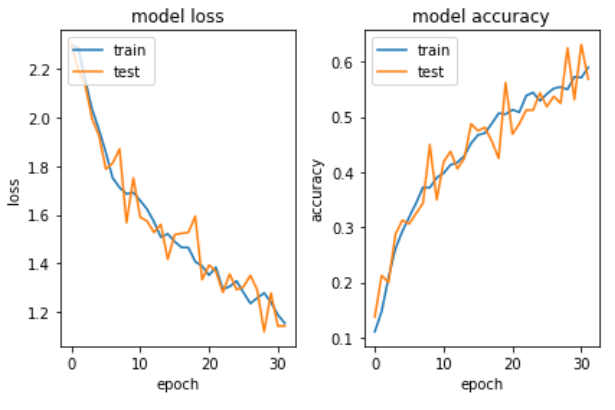
\includegraphics[width=250px]{sections/exp-1/images/model-1-acc.png}
    \captionof{figure}{Model 1 - Loss \& Accuracy}
\end{center}
